\documentclass{article}
%%%%%%%%%%%%%%%%%%%%%%%%%%%%%%%%%%%%%%%%%
% Lachaise Assignment
% Structure Specification File
% Version 1.0 (26/6/2018)
%
% This template originates from:
% http://www.LaTeXTemplates.com
%
% Authors:
% Marion Lachaise & François Févotte
% Vel (vel@LaTeXTemplates.com)
%
% License:
% CC BY-NC-SA 3.0 (http://creativecommons.org/licenses/by-nc-sa/3.0/)
% 
%%%%%%%%%%%%%%%%%%%%%%%%%%%%%%%%%%%%%%%%%

%----------------------------------------------------------------------------------------
%	PACKAGES AND OTHER DOCUMENT CONFIGURATIONS
%----------------------------------------------------------------------------------------

\usepackage{amsmath,amsfonts,stmaryrd,amssymb,subcaption} % Math packages

\usepackage{enumerate} % Custom item numbers for enumerations

\usepackage[ruled]{algorithm2e} % Algorithms

\usepackage[framemethod=tikz]{mdframed} % Allows defining custom boxed/framed environments

\usepackage{listings} % File listings, with syntax highlighting
\lstset{
	basicstyle=\ttfamily, % Typeset listings in monospace font
}

%----------------------------------------------------------------------------------------
%	DOCUMENT MARGINS
%----------------------------------------------------------------------------------------

\usepackage{geometry} % Required for adjusting page dimensions and margins

\geometry{
	paper=a4paper, % Paper size, change to letterpaper for US letter size
	top=2cm, % Top margin
	bottom=2.5cm, % Bottom margin
	left=2cm, % Left margin
	right=2cm, % Right margin
	headheight=14pt, % Header height
	footskip=1.5cm, % Space from the bottom margin to the baseline of the footer
	headsep=1.2cm, % Space from the top margin to the baseline of the header
	%showframe, % Uncomment to show how the type block is set on the page
}

%----------------------------------------------------------------------------------------
%	FONTS
%----------------------------------------------------------------------------------------

\usepackage[utf8]{inputenc} % Required for inputting international characters
\usepackage[T1]{fontenc} % Output font encoding for international characters

\usepackage{XCharter} % Use the XCharter fonts

%----------------------------------------------------------------------------------------
%	COMMAND LINE ENVIRONMENT
%----------------------------------------------------------------------------------------

% Usage:
% \begin{commandline}
%	\begin{verbatim}
%		$ ls
%		
%		Applications	Desktop	...
%	\end{verbatim}
% \end{commandline}

\mdfdefinestyle{commandline}{
	leftmargin=10pt,
	rightmargin=10pt,
	innerleftmargin=15pt,
	middlelinecolor=black!50!white,
	middlelinewidth=2pt,
	frametitlerule=false,
	backgroundcolor=black!5!white,
	frametitle={Command Line},
	frametitlefont={\normalfont\sffamily\color{white}\hspace{-1em}},
	frametitlebackgroundcolor=black!50!white,
	nobreak,
}

% Define a custom environment for command-line snapshots
\newenvironment{commandline}{
	\medskip
	\begin{mdframed}[style=commandline]
}{
	\end{mdframed}
	\medskip
}

%----------------------------------------------------------------------------------------
%	FILE CONTENTS ENVIRONMENT
%----------------------------------------------------------------------------------------

% Usage:
% \begin{file}[optional filename, defaults to "File"]
%	File contents, for example, with a listings environment
% \end{file}

\mdfdefinestyle{file}{
	innertopmargin=1.6\baselineskip,
	innerbottommargin=0.8\baselineskip,
	topline=false, bottomline=false,
	leftline=false, rightline=false,
	leftmargin=2cm,
	rightmargin=2cm,
	singleextra={%
		\draw[fill=black!10!white](P)++(0,-1.2em)rectangle(P-|O);
		\node[anchor=north west]
		at(P-|O){\ttfamily\mdfilename};
		%
		\def\l{3em}
		\draw(O-|P)++(-\l,0)--++(\l,\l)--(P)--(P-|O)--(O)--cycle;
		\draw(O-|P)++(-\l,0)--++(0,\l)--++(\l,0);
	},
	nobreak,
}

% Define a custom environment for file contents
\newenvironment{file}[1][File]{ % Set the default filename to "File"
	\medskip
	\newcommand{\mdfilename}{#1}
	\begin{mdframed}[style=file]
}{
	\end{mdframed}
	\medskip
}

%----------------------------------------------------------------------------------------
%	NUMBERED QUESTIONS ENVIRONMENT
%----------------------------------------------------------------------------------------

% Usage:
% \begin{question}[optional title]
%	Question contents
% \end{question}

\mdfdefinestyle{question}{
	innertopmargin=1.2\baselineskip,
	innerbottommargin=0.8\baselineskip,
	roundcorner=5pt,
	nobreak,
	singleextra={%
		\draw(P-|O)node[xshift=1em,anchor=west,fill=white,draw,rounded corners=5pt]{%
		Question \theQuestion\questionTitle};
	},
}

\newcounter{Question} % Stores the current question number that gets iterated with each new question

% Define a custom environment for numbered questions
\newenvironment{question}[1][\unskip]{
	\bigskip
	\stepcounter{Question}
	\newcommand{\questionTitle}{~#1}
	\begin{mdframed}[style=question]
}{
	\end{mdframed}
	\medskip
}

%----------------------------------------------------------------------------------------
%	WARNING TEXT ENVIRONMENT
%----------------------------------------------------------------------------------------

% Usage:
% \begin{warn}[optional title, defaults to "Warning:"]
%	Contents
% \end{warn}

\mdfdefinestyle{warning}{
	topline=false, bottomline=false,
	leftline=false, rightline=false,
	nobreak,
	singleextra={%
		\draw(P-|O)++(-0.5em,0)node(tmp1){};
		\draw(P-|O)++(0.5em,0)node(tmp2){};
		\fill[black,rotate around={45:(P-|O)}](tmp1)rectangle(tmp2);
		\node at(P-|O){\color{white}\scriptsize\bf !};
		\draw[very thick](P-|O)++(0,-1em)--(O);%--(O-|P);
	}
}

% Define a custom environment for warning text
\newenvironment{warn}[1][Warning:]{ % Set the default warning to "Warning:"
	\medskip
	\begin{mdframed}[style=warning]
		\noindent{\textbf{#1}}
}{
	\end{mdframed}
}

%----------------------------------------------------------------------------------------
%	INFORMATION ENVIRONMENT
%----------------------------------------------------------------------------------------

% Usage:
% \begin{info}[optional title, defaults to "Info:"]
% 	contents
% 	\end{info}

\mdfdefinestyle{info}{%
	topline=false, bottomline=false,
	leftline=false, rightline=false,
	nobreak,
	singleextra={%
		\fill[black](P-|O)circle[radius=0.4em];
		\node at(P-|O){\color{white}\scriptsize\bf i};
		\draw[very thick](P-|O)++(0,-0.8em)--(O);%--(O-|P);
	}
}

% Define a custom environment for information
\newenvironment{info}[1][Info:]{ % Set the default title to "Info:"
	\medskip
	\begin{mdframed}[style=info]
		\noindent{\textbf{#1}}
}{
	\end{mdframed}
}
 % Include the file specifying the document structure and custom commands
\setlength\parindent{0pt}
\usepackage[]{algorithm2e}
\usepackage{algpseudocode}

\title{EECS 545: Homework \#5} % Title of the assignment

\author{Mingliang Duanmu\\ \texttt{duanmuml@umich.edu}} % Author name and email address

\date{\today} % University, school and/or department name(s) and a date

\begin{document}

\maketitle % Print the title

\section{K-means for image compression}

\subsection*{a}

Refer to \textbf{\texttt{q1.py}}.

\subsection*{b}

Refer to \textbf{\texttt{q1.py}}.

\subsection*{c}

\begin{figure}[htbp]
    \centering
    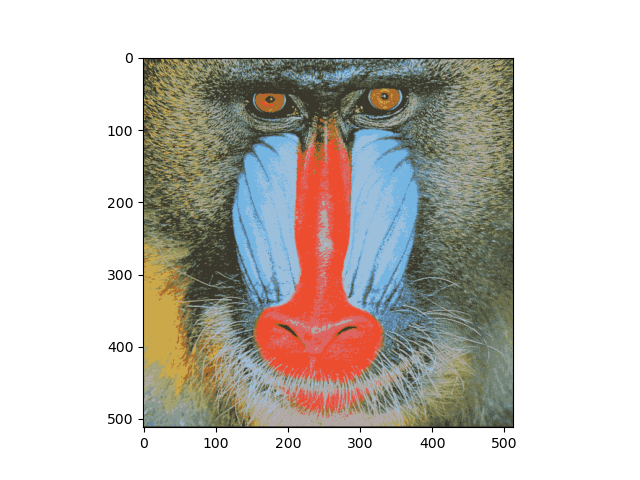
\includegraphics[width=.6\textwidth]{q1.png}
\end{figure}
The error is 15.068.

\subsection*{d}

0.83.

\newpage

\section{Gaussian mixtures for image compression}

\subsection*{a}

Refer to \textbf{\texttt{q2.py}}, log-likelihoods are displayed in output.

\subsection*{b}

Refer to \textbf{\texttt{q2.py}}.

\subsection*{c}

\begin{figure}[htbp]
    \centering
    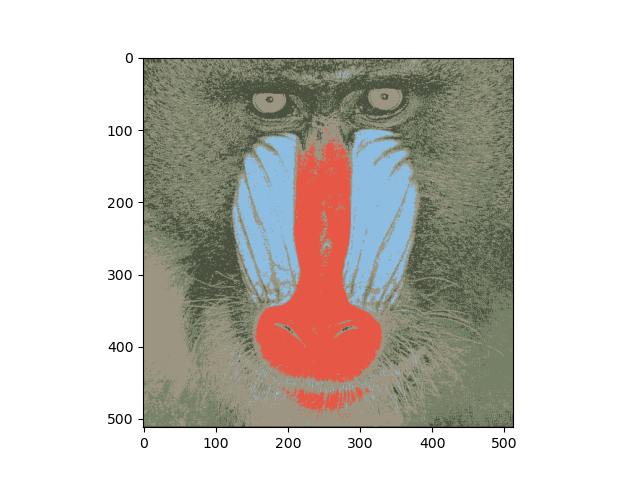
\includegraphics[width=.6\textwidth]{q2.png}
\end{figure}
The error is 33.227. $(\mu_k, \Sigma_k)$ are displayed in output. 

\subsection*{d}

0.875.

\newpage

\section{PCA and eigenfaces}

\subsection*{a}

We have 
$$
\begin{aligned}
\frac{1}{N} \sum_{n=1}^{N}\left\|x^{(n)}-U U^{T} x^{(n)}\right\|^{2} &=\frac{1}{N} \sum_{n=1}^{N}\left[\left(x^{(n)}-U U^{T} x^{(n)}\right)^{T}\left(x^{(n)}-U U^{T} x^{(n)}\right)\right] \\
&=\frac{1}{N} \sum_{n=1}^{N}\left[x^{(n) T} x^{n}-2 x^{(n) T} U U^{T} x^{(n)}+x^{(n) T} U U^{T} U^{T} U x^{(n)}\right]
\end{aligned}
$$
Because ${U_1, U_2, U_3, \cdots, U_K}$ are orthonormal, $U^TU = I$, we can simplify the result as
$$
\begin{aligned}
\frac{1}{N} \sum_{n=1}^{N}\left\|x^{(n)}-U U^{\top} x^{(n)}\right\|^{2} &=\frac{1}{N} \sum_{n=1}^{N}\left[x^{(n) T} x^{n}-x^{(n) T} U U^{T} x^{(n)}\right] \\
&=\frac{1}{N} \sum_{n=1}^{N}\left[x^{(n) T} x^{n}\right]-\frac{1}{N} \sum_{n=1}^{N}\left[x^{(n) T} U U^{T} x^{(n)}\right]
\end{aligned}
$$
Since $\sum_{n=1}^{N} x^{(n) T}x^n$ is constant, we can write the objective function as 
$$
\begin{aligned}
\max \frac{1}{N} \sum_{n=1}^{N}\left[x^{(n) T} U U^{T} x^{(n)}\right] &=\max \frac{1}{N} \sum_{n=1}^{N}\left\|U^{T} x^{(n)}\right\|^{2} \\ 
&=\max \frac{1}{N} \sum_{i=1}^{K} \sum_{n=1}^{N} u_{i}^{T} x^{(n)} x^{(n) T} u_{i}
\end{aligned}
$$
Since the data is zero-centered, we can simplify the covariance as
$$
S=\frac{1}{N} \sum_{n=1}^{N}\left(x^{(n)}-\bar{x}\right)\left(x^{(n)}-\bar{x}\right)^{T}=\frac{1}{N} \sum_{n=1}^{N}\left(x^{(n)}\right)\left(x^{(n)}\right)^{T}
$$
So the objective function becomes
$$
\max \sum_{i=1}^{K}u_i^TSu_i = \max \sum_{i=1}^{K}u_i^TSu_i + \lambda_i(1-u_i^Tu_i)
$$
where $u_i^Tu_i=1$
Compute the gradient and set to zero, we find
$$
Su_i = \lambda_iu_i
$$
which satisfies the definition of eigenvalues, $\lambda_i$ are the eigenvalues of the covariance matrix $S$ and $u_i$ are the corresponding eigenvectors. At the same time, we have 
$$
\max \sum_{i=1}^{K}u_i^TSu_i = \sum_{i=1}^K \lambda_i
$$
Therefore, we have
$$
\frac{1}{N} \sum_{n=1}^{N}\left[x^{(n) T} x^{n}\right]=\frac{1}{N} \sum_{n=1}^{N}\left\|x^{(n)}\right\|^{2}=\frac{1}{N} \sum_{n=1}^{N}\left\|V^{T} x^{(n)}\right\|^{2}
$$
where $V$ is orthogonal matrix. \\
Let $V$ be the eigenvectors of the covariance matrix, we have
$$
\begin{aligned}
\frac{1}{N} \sum_{n=1}^{N}\left\|V^{T} x^{(n)}\right\|^{2}&=\frac{1}{N} \sum_{i=1}^{d} \sum_{n=1}^{N} v_{i}^{T} x^{(n)} x^{(n) T} v_{i} \\ &=\sum_{i=1}^{d} v_{i}^{T} S v_{i} \\ &=\sum_{i=1}^{d} \lambda_{i}
\end{aligned}
$$
Finally we can conclude that
$$
\min _{\mathbf{U} \in \mathcal{U}} \frac{1}{N} \sum_{n=1}^{N}\left\|\mathbf{x}^{(n)}-\mathbf{U U}^{T} \mathbf{x}^{(n)}\right\|^{2}=\min _{\mathbf{U} \in \mathcal{U}} \frac{1}{N} \sum_{n=1}^{N}\left\|\mathbf{x}^{(n)}-\sum_{i=1}^{K} \mathbf{u}_{i} \mathbf{u}_{i}^{T} \mathbf{x}^{(n)}\right\|^{2}=\sum_{k=K+1}^{d} \lambda_{k}
$$

\subsection*{b}

\begin{figure}[htbp]
    \centering
    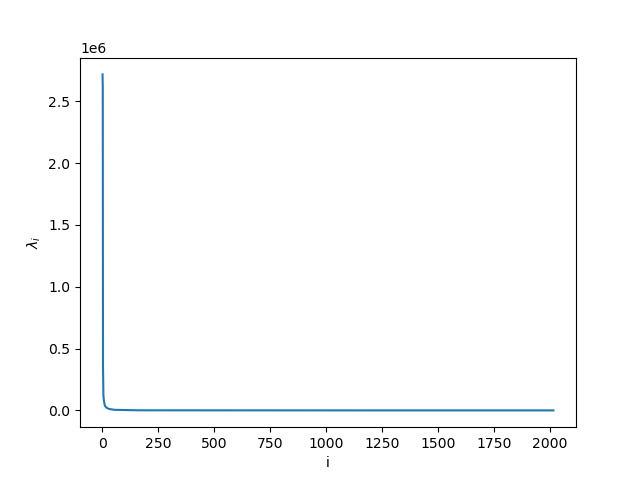
\includegraphics[width=.6\textwidth]{q31.png}
\end{figure}

\subsection*{c}

\begin{figure}[htbp]
    \centering
    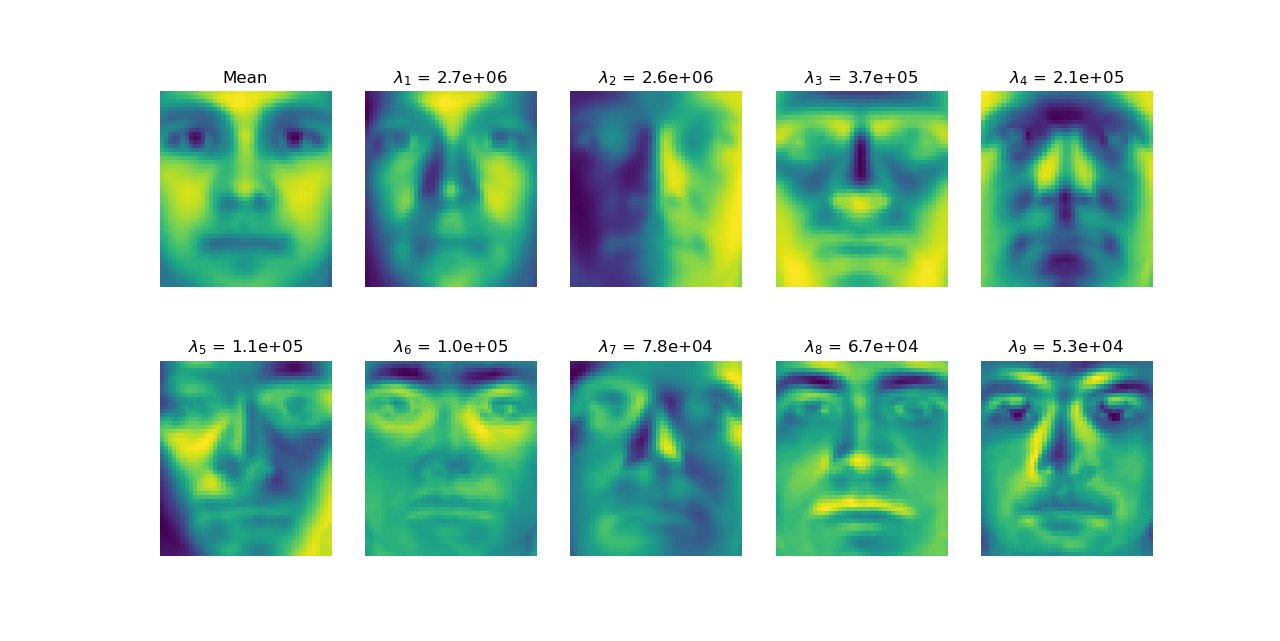
\includegraphics[width=.9\textwidth]{q32.png}
\end{figure}
The fourth principal component captures the light variations on sides of nose; the sixth principal component captures the light variations around the eyes; the eighth principal component captures the feature of lips.

\subsection*{d}

43 principal components are needed to represent 95\% of the total variance, 97.9\% of reduction in dimension. \\
167 principal components are needed to represent 99\% of the total variance, 91.7\% of reduction in dimension.

\newpage

\section{Expectation Maximization}

\subsection*{a}

The marginal distribution of $x$ looks like a normal distribution but with higher peak and longer tails.

\subsection*{b}

First we get the joint probability
$$
\begin{aligned}
P(x \mid \theta) &=\prod_{i=1}^{N} p(z) N\left(x \mid \mu, z, \sigma^{2}\right) \\
&=\phi^{N_{0}} \pi \frac{1}{\sqrt{2 \pi \sigma^{2}}} \exp \left(-\frac{1}{2 \sigma^{2}}(x-\mu)^{2}\right)(1-\phi)^{N_{1}} \pi \frac{1}{\sqrt{2 \pi \sigma^{2}}} \exp \left(-\frac{1}{2 \sigma^{2}}(\lambda-1-\mu)^{2}\right) \\
&=\phi^{N_{0}}(1-\phi)^{N_{1}} \prod_{i=1}^{N} \frac{1}{\sqrt{2 \pi \sigma^{2}}} \exp \left(-\frac{1}{2 \sigma^{2}}\left(x^{n}-z^{n}-\mu\right)^{2}\right)
\end{aligned}
$$
Converting to log likelihood, we have
$$
\log P(x \mid \theta)=N_{0} \log \phi+N_{1} \log (1-\phi)+\sum_{i=1}^{N}\left(\log \frac{1}{\sqrt{2 \pi}}-\log \sigma-\frac{1}{2 \sigma^{2}}\left(x^{n}-z^{n}-\mu\right)^{2}\right)
$$
To maximize the likelihood, we derive the gradient as
$$
\frac{\partial \log p}{\partial \phi}=\frac{N_{0}}{\phi}-\frac{N_{1}}{1-\phi}=0
$$
where $N_0$ corresponds to number when $z = 0$, same applies for $N_1$. \\
Therefore,
$$\phi=\frac{N_{\Omega}}{N_0+N_1}$$
Similarly, we have
$$
\frac{\partial \log P}{\partial \mu}=\sum_{i=1}^{N} \frac{1}{\sigma^{2}}\left(x^{n}-z^{n}-\mu\right)=0 
$$
$$
\frac{\partial \log P}{\partial \sigma}=\sum_{i=1}^{N}\left(-\frac{1}{\sigma}+\frac{1}{\sigma^{3}}\left(x^{n}-z^{n}-\mu\right)^{2}\right)=0
$$
Therefore, we get
$$\mu = \frac{\sum_{i=1}^{N}\varepsilon_i}{N} \quad \sigma^2 = \frac{1}{N}\sum_{i=1}^{N}(\varepsilon^n-\mu)^2$$

\subsection*{c}

According to EM, we have
$$
\log P(\boldsymbol{x} \mid \theta)=\sum_{\boldsymbol{z}} q(\boldsymbol{z}) \log \frac{p(\boldsymbol{z}, \boldsymbol{x} \mid \theta)}{q(\boldsymbol{z})}+K L(q(\boldsymbol{z}) \| p(\boldsymbol{z} \mid \boldsymbol{x}, \theta))
$$
For the E-step,
$$
q^{n}\left(z_{k}\right) =P\left(z_{k} \mid x^{n}\right)=\frac{P\left(z_{k}, x^{n}\right)}{P\left(x^{n}\right)} =\frac{\pi_{k} \phi_{k} N\left(x^{n} \mid \mu_{k}, \sigma_{k}\right)}{\sum_{k=1}^{K} \pi_{k} \phi_{k} N\left(x^{n} \mid \mu_{k}, \sigma_{k}\right)}=\gamma\left(z_{n k}\right)
$$
For the M-step,
$$
\begin{aligned}
\operatorname{argmax} & \sum_{\theta} \sum_{z} \gamma\left(z_{n k}\right) \log \left(z_{1}^{n} \mid \theta\right) \\
&=\sum_{n=1}^{N} \sum_{k=1}^{k} \gamma\left(z_{n k}\right) \log \left(z_{k}, x^{n} \mid \phi_{k}, \mu_{k}, \sigma_{k}\right) \\
&=\sum_{n=1}^{N} \sum_{k=1}^{k} \gamma\left(z_{n k}\right)\left(\log \pi_{k}+\log \phi_{k}-\frac{1}{2} \log (2 \pi)-\log \sigma_{k}-\frac{1}{2}\left(\frac{x^{n}-\mu_{k}}{\sigma_{k}}\right)^{2}\right)
\end{aligned}
$$
We need to derive the gradient of the parameters. \\
For $\pi_k$, the case is the same as in the lecture slides,
$$\pi_k = \frac{\sum_{n=1}^{N} \gamma\left(z_{n k}\right)}{N}$$
Since $\phi_0 + \phi_1 = 1$, 
$$
\frac{\partial J}{\partial \phi}=\sum_{n=1}^{N} \gamma\left(z_{n 0}\right) \frac{1}{\phi_{0}}-\gamma\left(z_{n 1}\right) \frac{1}{1-\phi_{0}}=0
$$
Therefore,
$$
\phi_{0}=\frac{\sum_{n=1}^{N} \gamma\left(z_{n 0}\right)}{\sum_{n=1}^{N} \gamma\left(z_{n 0}\right)+\gamma\left(z_{n 1}\right)}
$$
Similarly, we have
$$
\frac{\partial J}{\mu_{k}}=\sum_{n=1}^{N} \gamma\left(z_{n k}\right) \frac{x^{n}-\mu_{k}}{\sigma_{k}}=0
$$
$$
\frac{\partial J}{\partial \sigma_{k}}=\sum_{n=1}^{N} \gamma\left(z_{n k}\right)\left[-\frac{1}{\sigma_{k}}+\left(\frac{x^{n}-\mu_{k}}{\sigma_{k}}\right)\left(\frac{x^{n}-\mu_{k}}{\sigma_{k}^{2}}\right)\right]=0
$$
Therefore, we get
$$
\mu_{k}=\frac{\sum_{n=1}^{N} \gamma\left(z_{n k}\right) x^{n}}{\sum_{n=1}^{N} \gamma\left(z_{n k}\right)} \quad 
\sigma_{k}^{2}=\frac{\sum_{n=1}^{N} \gamma\left(z_{n k}\right)\left(x^{n}-\mu_{k}\right)^{2}}{\sum_{n=1}^{N} \gamma\left(z_{n k}\right)}
$$

\subsection*{d}

The addition of $\lambda$ makes $x$ possible for an arbitrary linear combination of two distributions, so the modified model is a generalized one that can be used to deal with more complicated real-world problems.

\newpage

\section{Independent Component Analysis}

\subsection*{a}

Refer to \textbf{\texttt{q5.py}} and the generated audio files.
 
\end{document}